\documentclass[a4paper,norsk, 10pt]{article}
\usepackage[utf8]{inputenc}
\usepackage{verbatim}
\usepackage{listings}
\usepackage{graphicx}
\usepackage[norsk]{babel}
\usepackage{a4wide}
\usepackage{color}
\usepackage{amsmath}
\usepackage{float}
\usepackage{amssymb}
\usepackage[dvips]{epsfig}
\usepackage[toc,page]{appendix}
\usepackage[T1]{fontenc}
\usepackage{cite} % [2,3,4] --> [2--4]
\usepackage{shadow}
\usepackage{hyperref}
\usepackage{titling}
\usepackage{marvosym }
\usepackage{subcaption}
\usepackage[noabbrev]{cleveref}
\usepackage{cite}


\setlength{\droptitle}{-10em}   % This is your set screw

\setcounter{tocdepth}{2}

\lstset{language=c++}
\lstset{alsolanguage=[90]Fortran}
\lstset{alsolanguage=Python}
\lstset{basicstyle=\small}
\lstset{backgroundcolor=\color{white}}
\lstset{frame=single}
\lstset{stringstyle=\ttfamily}
\lstset{keywordstyle=\color{red}\bfseries}
\lstset{commentstyle=\itshape\color{blue}}
\lstset{showspaces=false}
\lstset{showstringspaces=false}
\lstset{showtabs=false}
\lstset{breaklines}
\title{FYS3140 Home exam}
\author{Kandidatnr. 15135}
\begin{document}
\maketitle

\section*{1)}

We have the differential equation

\begin{equation}
t^2 \frac{d^2u}{dt^2} - t\frac{du}{dt} + u = t
\end{equation}

This is on the form of a Euler-Cauchy equation, meaning that we can solve it by doing the change of variable:

$$
t = e^z, \qquad \frac{dz}{dt} = \frac{1}{t} \qquad (t>0)
$$
$$
t = -|t| = -e^z, \qquad \frac{dz}{dt} = \frac{1}{t} \qquad (t<0)
$$

From $\frac{dz}{dt} = \frac{1}{t}$ we see that $t \neq 0$. After the change of variable the differential equation takes the form

\begin{equation}
\frac{d^2u}{dz^2} + (-1 -1)\frac{du}{dz} + u = e^z
\label{eq:transformed_DE}
\end{equation}

So is a inhomogeneous 2. order ODE, and is easy to solve. We have to do it in 2 steps. We will first find the homogeneous solution $u_h$, and then a particular solution $u_p$. From these we can find the general solution.\\

$\underline{\mathbf{u_h}}$:\\

The homogeneous equation is:

$$
u'' - 2u' + u = 0
$$

Using the ansatz that the solution is on the form $e^{\lambda z}$ we get the characteristic polynomial:

$$
\lambda^2 -2\lambda + 1 = 0
$$

The solution(s) is

$$
\lambda = \frac{2 \pm \sqrt{4-4}}{2} = 1
$$

The characteristic polynomial has only one solution $\lambda = 1$, giving us the solution $u_1(z) = Ae^z$. But to span the entire solution space of the differential equation we need two linear independent solutions. From the variation of parameters we know that we can construct such an solution be multiplying the first solution by $z$, giving us $u_2(z) = Bze^z$. Since we now have two solutions we can write down the homogeneous solution:

\begin{equation}
u_h(z) = Ae^z + Bze^z
\end{equation}

We can now find a particular solution: \\

\newpage

$\underline{\mathbf{u_p}}$:\\

We now have to look at 

$$
u'' - 2u' + u = e^z
$$

We are going to make a "guess" for the 	particular solution. We are going to make the guess that the solution is on the form $u_p = Q_n e^z$, where $Q_n$ is a polynomial of degree $n$. The particular solution can not be on the same form as the general solution, so it can not be on the form $e^z$ nor $ze^z$. The smartest guess is $Q_2 e^z$, and the easiest polynomial of degree 2 is $Cz^2$, so we are going to guess:

$$
u_p(z) = Cz^2e^z
$$ 

We need the derivatives:

$$
u_p' = C(2ze^z + z^2e^z), \qquad u_p'' = C(2e^z + 4ze^z + z^2e^z)
$$

We can so insert this back into the differential equation:

$$
u'' - 2u' + u = C(2e^z + 4ze^z +z^2e^z - 4ze^z - 2z^2e^z + z^2e^z) = e^z
$$

Most of the terms disappears, and we get:

$$
2Ce^z = e^z \Rightarrow C = \frac{1}{2}
$$

Giving us the particular solution

$$
u_p(z) = \frac{1}{2}z^2 e^z
$$

We now have all we need to find the general solution:

$$
u(z) = u_h(z) + u_p(z) = Ae^z + Bze^z + \frac{1}{2}z^2 e^z
$$

But this is only the solution for \ref{eq:transformed_DE}. We need to change the variable back to the original variable. But since we can have both negative and positive $t$ we are going to use $|t|$ in the general solution. We use that

$$
z = \ln |t|
$$

We now get the correct general solution:

\begin{equation}
\underline{u(t) = \tilde{A}t + \tilde{B}t\ln |t| + \frac{1}{2}t \ln |t|^2}
\end{equation}


We can now apply the initial conditions $u(1) = 1$, $u(e) = e$:

$$
u(1) = \tilde{A} = 1 
$$
$$
u(e) = \tilde{A}e + \tilde{B}e + \frac{1}{2}e = e \Rightarrow \tilde{B} = -\frac{1}{2}
$$

This gives us the final solution:

\begin{equation}
\underline{\underline{u(t) = t -\frac{1}{2}t\ln |t| + \frac{1}{2}t\ln |t|^2}}
\end{equation}
\newpage

\section*{2)}

\subsection*{b)}
\begin{figure}[H]
\centering
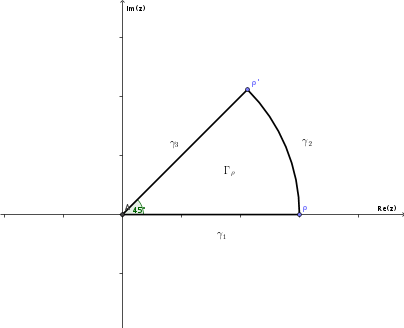
\includegraphics[scale=0.8]{2b.png}
\caption{A drawing of the contour $\Gamma_{\rho}$. $\gamma_1$ goes from $z = x=0$ to $z = x = \rho$. $\gamma_2$ goes from $z = \rho$ to $z = \rho e^{i\pi/4}$. $\gamma_3$ goes from $z = \rho e^{i\pi/4}$ and back to the origin.}
\end{figure}

We have the contour integral

$$
\tilde{I} = \int_{\Gamma_{\rho}} e^{iz^2}dz
$$

We see that for every $\rho$ $e^{iz^2}$ is analytic; $e^{iz^2}$ is well-defined and has no singularities for the entire $\mathbb{C}$. The Cauchy Theorem says that if a function $f(z)$ is analytic inside and on a contour $\Gamma$ when

$$
\int_{\Gamma} f(z) dz = 0
$$

Since $e^{iz^2}$ is analytic inside and on $\Gamma_{\rho}$ then:

$$
\underline{\underline{\tilde{I} = \int_{\Gamma_{\rho}} e^{iz^2}dz = 0}}
$$

\subsection*{c)}

The integral

$$
\tilde{I}_1 = \int_{\gamma_1} e^{iz^2} dz = int_0^{\rho} e^{iz^2} dz
$$

is a integral over a line on the real axis, so to make this an integral of a real value we are going to do the trivial transformation:

$$
z = x, \qquad dz = dx
$$

And for the boundaries

$$
0 \rightarrow 0, \qquad \rho \rightarrow \rho
$$

So the integral becomes

$$
\int_{\gamma_1} e^{iz^2} dz \rightarrow \int_0^{\rho} e^{ix^2}dx
$$

This is closely connected to out original integral $I$. As $\rho$ becomes larger and larger, $\int_0^{\rho} e^{ix^2}dx$ comes closer and closer to $I$. So:

\begin{equation}
I = \lim_{\rho \rightarrow \infty} \int_0^{\rho} e^{ix^2}dx = \lim_{\rho \rightarrow \infty} \int_0^{\rho} e^{iz^2}dz
\label{eq:I1}
\end{equation}


\subsection*{d)}

We have the integral

$$
\tilde{I}_ 3 = \int_{\gamma_3}e^{iz^2} dz = \int_{\rho e^{i\pi/4}}^0 e^{iz^2} dz 
$$

We have to make a change of variables. We are interested in getting simpler boundary conditions, so a way to make the $e^{i\pi/4}$ the lower boundary disappear would give a good ansatz. So we are going to try:

$$
x = e^{-i\pi/4}z. \qquad dx = e^{-i\pi /4}dz
$$

The boundaries then becomes:

$$
z = \rho e^{i\pi/4} \rightarrow x = \rho, \qquad z = 0 \rightarrow x = 0
$$

We then look at the integrand:

$$
e^{iz^2} = e^{i(e^{i\pi/4}x)^2} = e^{ie^{i\pi/2}x^2} = e^{i\cdot ix^2} = e^{-x^2}
$$

This gives 

$$
\tilde{I}_3 = \int_{\rho}^0 e^{-x^2} e^{i\pi /4} dx = - \int_0^{\rho} e^{-x^2} e^{i\pi /4} dx
$$

We know that 

$$
e^{i\pi/4} =\frac{1+i}{\sqrt{2}}
$$

This gives us the final result:

\begin{equation}
\int_{\gamma_3}e^{iz^2} dz = -\frac{1+i}{\sqrt{2}}\int_0^{\rho}e^{-x^2}dx
\label{eq:I3}
\end{equation}



\subsection*{e)}

\subsection*{f)}

We can now use all the above to find the integral $I$. We know that

$$
\tilde{I} = \tilde{I}_1 + \tilde{I}_2 + \tilde{I}_3 = 0
$$

We are interested in the case where $\rho$ goes to infinity. We are going to look at all the terms of the expression one by one, and see how they behave as $\rho$ goes to infinity.\\

$\underline{\mathbf{\tilde{I}}}$:\\

$\tilde{I} = 0$ independently of $\rho$, so
\begin{equation}
\lim_{\rho \rightarrow \infty} \tilde{I} = 0
\label{eq:IrhoInf}
\end{equation}\\

$\underline{\mathbf{\tilde{I}_1}}$:\\

We saw from \ref{eq:I1} that

\begin{equation}
\lim_{\rho \rightarrow \infty} \tilde{I}_1 = \lim_{\rho \rightarrow \infty} \int_0^{\rho} e^{ix^2} dx = I
\label{eq:I1rhoInf}
\end{equation}\\

$\underline{\mathbf{\tilde{I}_2}}$:\\

We found that

$$
\bigg|\int_{\gamma_2}e^{iz^2}dz \bigg| \leq \frac{\pi}{4\rho}
$$

We can look at this upper bound. It is easy to see that

$$
\lim_{\rho\rightarrow \infty} \frac{\pi}{4\rho} = 0
$$
So we get that

$$
\lim_{\rho \rightarrow \infty } \bigg|\int_{\gamma_2}e^{iz^2}dz \bigg| \leq 0
$$

But since $\big|\int_{\gamma_2}e^{iz^2}dz \big|$ has to be positive, we get that

$$
\lim_{\rho \rightarrow \infty } \bigg|\int_{\gamma_2}e^{iz^2}dz \bigg| = 0
$$

If the length of the integral is zero, then the integral has to be zero, so:

\begin{equation}
\lim_{\rho \rightarrow \infty} \tilde{I}_2 = \lim_{\rho \rightarrow \infty}  \int_{\gamma_2}e^{iz^2}dz = 0
\label{I2rhoInf}
\end{equation}\\

$\underline{\mathbf{\tilde{I}_3}}$:\\

For the last integral we have that 

$$
\lim_{\rho \rightarrow \infty}  \int_{\gamma_3}e^{iz^2}dz = \lim_{\rho \rightarrow \infty} -\frac{1+i}{\sqrt{2}}  \int_0^{\rho}e^{-x^2}dx 
$$

We can look at the last part of that integral:

$$
\lim_{\rho \rightarrow \infty} \int_0^{\rho}e^{-x^2}dx  = \int_0^{\infty}e^{-x^2}dx
$$

This is a know integral we can look up in Rottman, where we find this to equal $\frac{\sqrt{\pi}}{2}$. So:

\begin{equation}
\lim_{\rho \rightarrow \infty} \tilde{I}_3 = \lim_{\rho \rightarrow \infty} \int_{\gamma_3}e^{iz^2}dz = \lim_{\rho \rightarrow \infty} -\frac{1+i}{\sqrt{2}}  \int_0^{\rho}e^{-x^2}dx = -\frac{1+i}{\sqrt{2}} \frac{\sqrt{\pi}}{2}
\label{I3rhoinf}
\end{equation}\\

We can now use all this to find the original integral $I$.

$$
\lim_{\rho \rightarrow \infty} \tilde{I} = \lim_{\rho \rightarrow \infty} \tilde{I}_1 + \lim_{\rho \rightarrow \infty} \tilde{I}_2 + \lim_{\rho \rightarrow \infty} \tilde{I}_3 = 0
$$

and by using \ref{eq:I1rhoInf}, \ref{I2rhoInf} and \ref{I3rhoinf} we find that

$$
\lim_{\rho \rightarrow \infty} \tilde{I} = I + 0 - \frac{1+i}{\sqrt{2}} \frac{\sqrt{\pi}}{2} = 0
$$

This gives us the final result:

$$
I = \int_0^{\infty}e^{ix^2}dx =\underline{\underline{\left(\frac{1}{2} +\frac{i}{2}\right) \sqrt{\frac{\pi}{2}}}}
$$\\

We can now use this to evaluate some integrals:

$$
\int_0^{\infty} \cos(x^2) dx = \int_0^{\infty} \frac{1}{2}(e^{ix^2} + e^{-ix^2}) dx  = \int_0^{\infty} \frac{1}{2}(e^{ix^2} + e^{i(ix)^2}) dx
$$
$$
= \frac{1}{2}\left(\left(\frac{1}{2} +\frac{i}{2}\right) \sqrt{\frac{\pi}{2}}  + \right)
$$



\section*{3)}
\subsection*{a)}

Fermat's principle is given by

\begin{equation}
P = \int_A^B n(r) ds
\end{equation}

For polar coordinates the line element $ds$ is given as 

$$
ds = \sqrt{dr^2 + r^2d\theta^2}
$$

Giving us the path

$$
P = \int_A^B n(r) \sqrt{dr^2 + r^2d\theta^2}
$$

Now, we have two alternatives, we can either put out $dr$ or $d\theta$ from the square root, giving us two different integrals:

\begin{equation}
P_1 = \int_A^B n(r)\sqrt{1 + r^2 \left(\frac{d\theta}{dr}\right)^2} dr
\label{eq:p1}
\end{equation}



and

\begin{equation}
P_2 = \int_A^B n(r)\sqrt{r^2 +  \left(\frac{dr}{d\theta}\right)^2} d\theta
\label{eq:p2}
\end{equation}



We are interested in the minima of these paths. This is a problem in calculus of variation, which we know how to solve. We can find the shortest path by the using Euler-Lagrange equation. If we look at $P_1$ we see that it has no explicit dependence on $\theta$. Meaning that if we write the Euler-Lagrange equation for $P_1$:

$$
\frac{d}{dr}\frac{\partial L}{\partial \theta'} - \frac{\partial L}{\partial \theta} = 0
$$ 

Where $L = n(r)\sqrt{1 + r^2 \left(\frac{d\theta}{dr}\right)^2}$.\\

We can see that the term $\frac{\partial L}{\partial \theta}$ disappears($\theta$ is a \textit{cyclic} variable). This gives us a much easier equation to solve, as the problem reduces from a second order, to a first order differential equation:

\begin{equation}
\frac{d}{dr}\frac{\partial L}{\partial \theta'} = 0 \Leftrightarrow \frac{\partial L}{\partial \theta'} = C
\label{eq:lagrange}
\end{equation}

Where $C$ is some constant.\\

This is now the case for $P_2$, which is explicitly dependent on $\theta$, $\theta'$ and $r$. So $P_1$ is the best choice.


\subsection*{b)}

We are now going to start to minimize the path of $P_1$ \ref{eq:p1}. As mentioned above this means we have to solve the Euler-Lagrange equation, which we showed reduces \ref{eq:lagrange} to

$$
\frac{\partial L}{\partial \theta'} = C
$$

Where

$$
L = n(r)\sqrt{1 + r^2 \left(\frac{d\theta}{dr}\right)^2}
$$

Taking the partial differentiation we get that:

$$
\frac{\partial L}{\partial \theta'} = n(r) \frac{r^2\theta'}{\sqrt{1 + r^2\theta'^2}} = C
$$

where $\theta' = \frac{d\theta}{dr}$. To solve this differential equation we need to clean up the expression, to make it possible to separate the variables. We start by taking the square of both sides:

$$
\Rightarrow n^2(r)\frac{r^4 \theta'^2}{1+r^2\theta'^2} = C^2 = D
$$

Then interchanging $D$ and $1+r^2\theta'^2$, and isolation $r^2\theta'^2$:

$$
\frac{n^2(r)}{D}r^4\theta'^2 = 1 + r^2\theta'^2
$$

$$
r^2\theta'^2\left(\frac{n^2(r)}{D}r^2 - 1\right) = 1
$$

Then moving $r^2\theta'^2$ to the RHS:

$$
\Rightarrow r^2\frac{n^2(r)}{D} - 1 = \frac{1}{r^2}\frac{1}{\theta'^2}
$$

We can see that 

$$
\frac{1}{\theta'^2} = \left(\frac{d\theta}{dr}\right)^{-2} = \left(\frac{dr}{d\theta}\right)^2
$$

So we get:

$$
\frac{1}{r^2}\left(\frac{dr}{d\theta}\right)^2 = r^2\frac{n^2(r)}{D} -1
$$

We now need to get rid of the constant $D$. We know that at the distance $d$ is the closes point in the path to the point $\mathcal{O}$, and thus we have that $\frac{\partial L}{\partial \theta} = 0$. We insert this in to the above expression to find $D$:


$$
\left(\frac{dr}{d\theta}\right)^2_{r = d} = 0 = d^2\frac{n^2(d)}{D} -1
$$

$$
\Rightarrow d^2\frac{n^2(d)}{D} = 1 \Leftrightarrow D = d^2 n^2(d)
$$

We can now eliminate $D$, and find that:

\begin{equation}
\underline{\underline{\frac{1}{r^2}\left(\frac{dr}{d\theta}\right)^2 = \frac{r^2}{d^2}\frac{n^2(r)}{n^2(d)} -1}}
\label{eq:sepDiff}
\end{equation}


\subsection*{c)}

Now we have a separable DE \ref{eq:sepDiff}. We are going to use that the refractive index is given as 

\begin{equation}
n(r) = \sqrt{1 + \frac{\kappa^2}{r^2}}
\label{eq:refIndex}
\end{equation}

This also gives us the refractive index at $d$ is given as

$$
n(d) = \sqrt{1 + \frac{\kappa^2}{d^2}}
$$

If we insert this into \ref{eq:sepDiff} we get that 

$$
\frac{1}{r^2}\left(\frac{dr}{d\theta}\right)^2 = \frac{r^2}{d^2}\frac{1 + \frac{\kappa^2}{r^2}}{1 + \frac{\kappa^2}{d^2}} -1
$$
$$
= \frac{r^2 + \kappa^2}{d^2+\kappa^2} - 1 = \frac{r^2 + \kappa^2}{d^2+\kappa^2} - \frac{d^2+\kappa^2}{d^2+\kappa^2} = \frac{r^2 -d^2}{d^2 +\kappa^2}
$$
So

$$
\left(\frac{dr}{d\theta}\right)^2 = r^2\frac{r^2 -d^2}{d^2 +\kappa^2}
$$


We are interested inn an expression for $\theta$, so we can write the above as:

\begin{equation}
d\theta = \frac{1}{r}\left(\frac{r^2 -d^2}{d^2 +\kappa^2}\right)^{-1/2}dr
\end{equation}


We are interested in finding how much the light is refracted when it moves from far way, gets refracted inside the medium, comes to a distance $d$ from $\mathcal{O}$ then move far way.

\begin{figure}[H]
\centering
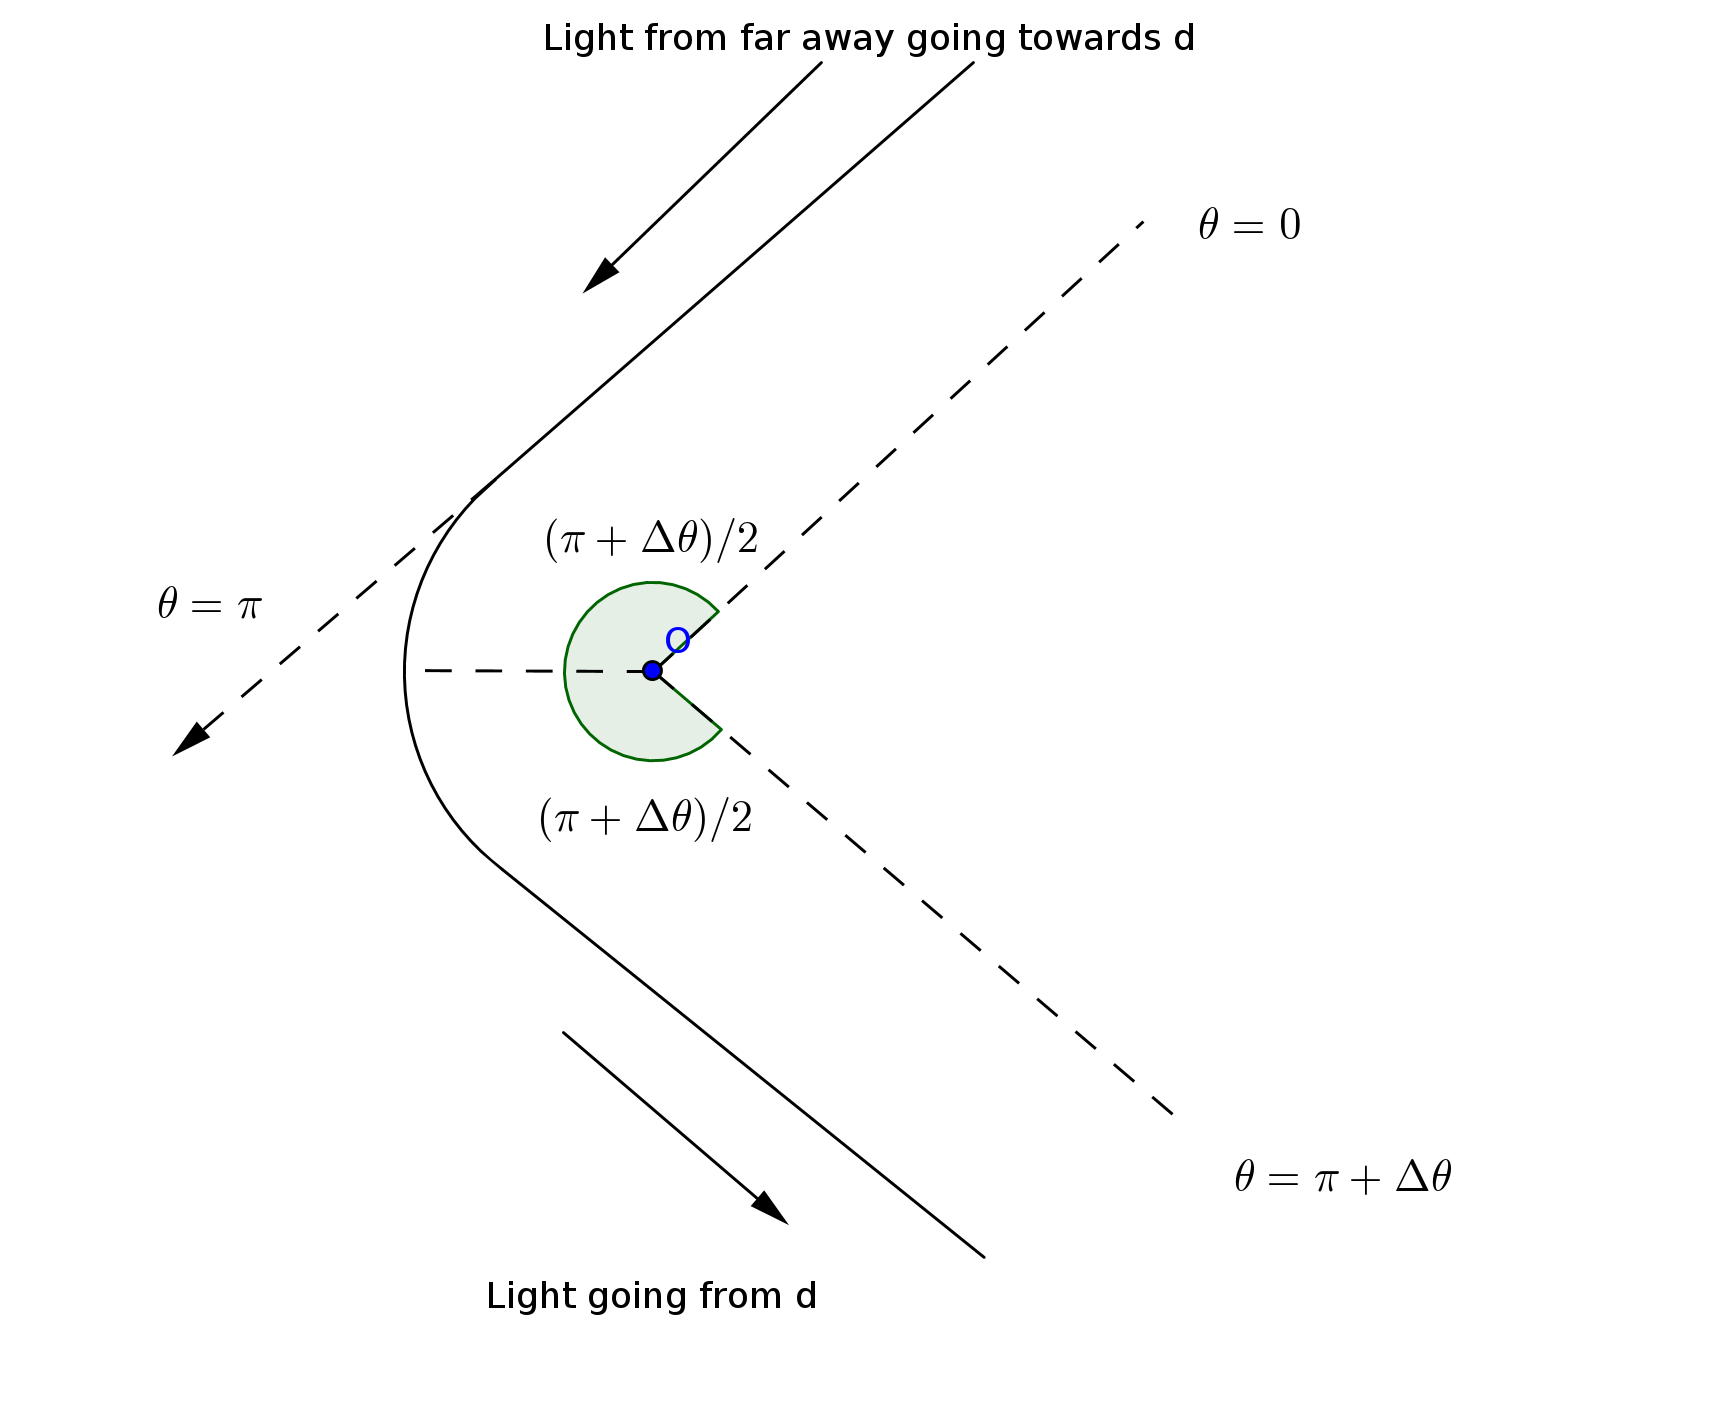
\includegraphics[scale=0.4]{3c.png}
\caption{A crude drawing of the light moving from far away to d, then away from $\mathcal{0}$. We can see that the light deflects the same amount on both the way in and the way out.}
\end{figure}

Since the refractive index is only dependent on the distance from $\mathcal{O}$ the deflection angle will be the same as the light moves in, as when it moves out. This means that we only have to find the angle form $r = d$ to $r = \infty$(I am going to set "far away" as meaning $r\rightarrow \infty$). So:

$$
\frac{\Delta \theta}{2} = \Delta\theta_{d\rightarrow \infty} = \int d\theta = \int_d^{\infty} \frac{1}{r}\left(\frac{r^2 -d^2}{d^2 +\kappa^2}\right)^{-1/2}dr
$$

$$
= \sqrt{d^2 +\kappa^2}\int_d^{\infty} \frac{1}{r\sqrt{r^2 - d^2}}dr
$$

We are going to use a change of variable:

$$
r = d \cosh x
$$

We find the Jacobi factor:

$$
\frac{dr}{dx} = d\sinh x \Leftrightarrow dr = d\sinh(x) dx
$$

Since we are changing variables we have to change the boundaries:

$$
\lim_{r\rightarrow \infty}\cosh^{-1} \frac{r}{d} = \infty, \qquad \cosh^{-1}\frac{d}{d} = 0
$$

We then get the integral:

$$
\Delta\theta_{d\rightarrow \infty} = \sqrt{d^2 +\kappa^2}\int_0^{\infty} \frac{d\sinh x}{d\cosh x\sqrt{d^2\cosh^2 x - d^2}}dx
$$

$$
= \frac{\sqrt{d^2 +\kappa^2}}{d}\int_0^{\infty} \tanh x \frac{1}{\sqrt{\cosh^2 x - 1}}dx
$$

We know that $\cosh^2 x - 1 = \sinh^2 x$, so since $\tanh x = \frac{\sinh x}{\cosh x}$ we get that:

$$
\Delta\theta_{d\rightarrow \infty} = \frac{\sqrt{d^2 +\kappa^2}}{d}\int_0^{\infty} \frac{1}{\cosh x}dx
$$

Using Rottman we find that this is:

$$
= \frac{\sqrt{d^2 +\kappa^2}}{d} (2 \arctan (\tanh \left(\frac{x}{2}\right))) \bigg|_0^{\infty}
$$

$$
= \frac{\sqrt{d^2 +\kappa^2}}{d} \frac{\pi}{2}
$$

And since the deflection angle of the incoming light is the same as the outgoing, we get that:

$$
\Delta \theta = \theta_{slutt} - \theta_{start} = 2\Delta\theta_{d\rightarrow\infty} = \underline{\underline{\pi \frac{\sqrt{d^2 +\kappa^2}}{d}}}
$$

\end{document}


